% =============================================================================
% Lecture 07: Introduction to Neural Networks (PyTorch)
% ECON 8310: Business Forecasting
% University of Nebraska at Omaha
% =============================================================================

\documentclass[aspectratio=169, 11pt]{beamer}

\input{header}

% ---- Lecture metadata --------------------------------------------------------
\title[Neural Networks]{Introduction to Neural Networks}
\subtitle{ECON 8310: Business Forecasting --- Lecture 7}
\author{Department of Economics}
\institute{University of Nebraska at Omaha}

% =============================================================================
\begin{document}
% =============================================================================

\begin{frame}
  \titlepage
\end{frame}

% ---- Outline ----------------------------------------------------------------
\begin{frame}{Lecture Outline}
  \tableofcontents
\end{frame}

% =============================================================================
\section{From Trees to Neural Networks}
% =============================================================================

\sectionslide{From Trees to Neural Networks}{%
  Trees predict in steps. Networks predict in curves --- and that difference
  buys less than you would expect on tabular data, and everything on sequences.}

% --- Slide: Motivation -------------------------------------------------------
\begin{frame}{Why Go Beyond Trees?}
  A tree treats rows as independent: time enters only as the lag columns you built. Its
  prediction is \textbf{piecewise constant}, so in Lab 4 it could not predict above the largest
  value it had seen.

  \vspace{0.15cm}
  A network's prediction is \textbf{continuous} --- with ReLU, piecewise linear.

  \begin{warningbox}
    \textbf{This is not an upgrade.} On Homeworks 3 and 4, boosting and a tuned LASSO were hard
    to beat; a network often loses to both. Reach for one for \emph{sequences}, images or audio,
    or very large $n$.
  \end{warningbox}
\end{frame}

% --- Slide: From regression to a neuron ---------------------------------------
\begin{frame}{From Linear Regression to a Single Neuron}
  Start from something you already know. Linear regression predicts
  $\hat{y} = \mathbf{w}^\top \mathbf{x} + b$.

  \vspace{0.15cm}
  A \textbf{neuron} is that same expression with one addition --- a nonlinear
  \textbf{activation} $\sigma(\cdot)$ wrapped around it:
  \[
    a = \sigma(\mathbf{w}^\top \mathbf{x} + b)
  \]
  \vspace{-0.45cm}
  \begin{center}
    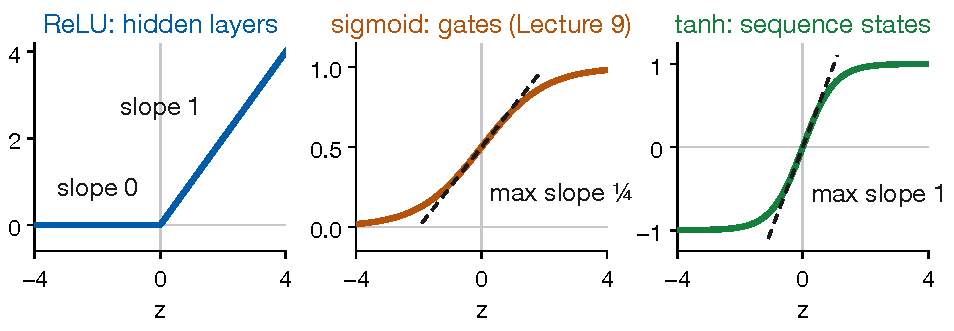
\includegraphics[height=3.7cm]{../Figures/Lecture07_NeuralNets/activation_slopes.pdf}
  \end{center}
  \vspace{-0.3cm}
  {\small The slopes matter in Lecture 9: each sigmoid scales a gradient passing back through it
  by at most $\frac{1}{4}$. A regression's output layer has no squashing at all: $\sigma(z) = z$.}
\end{frame}

% --- Slide: why nonlinearity ---------------------------------------------------
\begin{frame}{Why the Nonlinearity Is the Whole Trick}
  Depth alone buys nothing: a linear function of a linear function is linear,
  $\mathbf{W}_2(\mathbf{W}_1\mathbf{x}) = (\mathbf{W}_2\mathbf{W}_1)\mathbf{x}$. Weekday
  electricity load against the day of the year:
  \begin{center}
    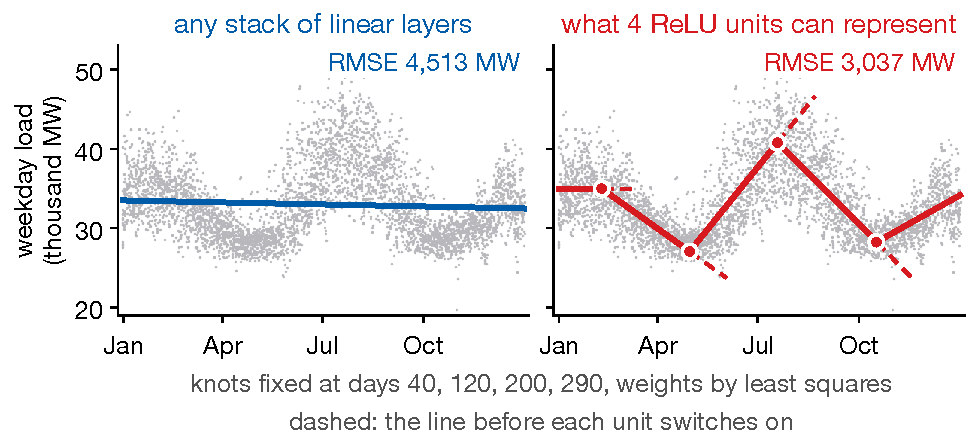
\includegraphics[height=4.6cm]{../Figures/Lecture07_NeuralNets/relu_hinges.pdf}
  \end{center}
  \vspace{-0.4cm}
  {\small With one input, a hidden layer of $H$ ReLU units draws a continuous, piecewise-linear
  curve with at most $H$ kinks: a linear spline whose knots the network learns. Prophet's trend
  (Lecture 3) is the same sum, with its changepoints fixed in advance.}
\end{frame}

% --- Slide: universal approximation -------------------------------------------
\begin{frame}{Universal Approximation: Existence, Not Estimation}
  Add units and the kinks multiply. With enough of them, one hidden layer can approximate
  \emph{any} continuous function arbitrarily well: the \textbf{universal approximation theorem}.

  \vspace{0.15cm}
  \textbf{Read it carefully.} It says a network \emph{can} represent the function --- not
  that your optimizer will find it, that you have the data to identify it, or that it will
  generalize.

  \vspace{0.15cm}
  Four units already reach RMSE 3{,}037 on the electricity year, and no function of the day of
  the year fits better than 2{,}864. Past that, capacity is not what is missing.
\end{frame}

% =============================================================================
\section{Feedforward Networks}
% =============================================================================

\sectionslide{Feedforward Networks}{%
  Stack layers of neurons, and each layer learns a higher-level
  representation of the one below it.}

% --- Slide: Layers and forward pass ------------------------------------------
\begin{frame}{Feedforward Network: Layers and Forward Pass}
  A \textbf{feedforward network} (FFN, or multilayer perceptron) is three things in sequence: an
  \textbf{input layer} of features $\mathbf{x} \in \mathbb{R}^p$; \textbf{hidden layers}, each
  applying
  $\mathbf{a}^{(\ell)} = \sigma\!\left(\mathbf{W}^{(\ell)}\mathbf{a}^{(\ell-1)} + \mathbf{b}^{(\ell)}\right)$;
  and a linear \textbf{output layer} for regression.

  \vspace{0.15cm}
  \textbf{Width} is the number of neurons in a layer, \textbf{depth} the number of hidden layers.

  \begin{keybox}
    \textbf{Sensible starting sizes for forecasting:} 2--3 hidden layers, 64--256 neurons each,
    ReLU, dropout 0.2--0.5. Start at the small end of every range.
  \end{keybox}

  \vspace{0.1cm}
  Add capacity only when validation error says the model is too simple.
\end{frame}

% --- Slide: counting parameters ------------------------------------------------
\begin{frame}{How Big Is This Model, Actually?}
  Capacity is easy to add by accident, so count it once: a layer mapping $m$ inputs to $n$ outputs
  holds $m \times n$ weights plus $n$ biases. Our weekly panel, 46 engineered features in, two
  hidden layers of 128, one output:
  \vspace{-0.2cm}
  \begin{center}
    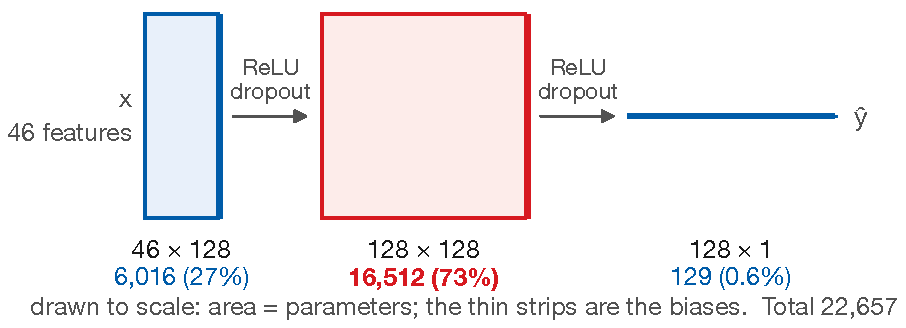
\includegraphics[height=3.9cm]{../Figures/Lecture07_NeuralNets/weight_blocks.pdf}
  \end{center}
  \vspace{-0.3cm}
  \textbf{Twenty-two thousand parameters on five thousand rows} --- four per observation, and
  the one $128 \times 128$ block holds 73\% of them. Lecture 6 called sixty predictors on 150
  rows a crisis; what makes this survivable is the regularization, next.
\end{frame}

% =============================================================================
\section{Training: Loss and Backpropagation}
% =============================================================================

\sectionslide{Training: Loss and Backpropagation}{%
  Compute the error, propagate it backward, adjust every weight
  by its share of the blame. Repeat.}

% --- Slide: Loss and SGD -----------------------------------------------------
\begin{frame}{Training: Loss, Gradients, and the Update Step}
  Training is one loop. \textbf{First}, the loss: for regression, mean squared error
  $\mathcal{L} = \frac{1}{n}\sum_i (y_i - \hat{y}_i)^2$. \textbf{Second, backpropagation:} the
  chain rule, run backward, gives each weight its share of the error. \textbf{Third}, step every
  weight against its gradient:
  \[
    \mathbf{W} \leftarrow \mathbf{W} - \eta \, \frac{\partial \mathcal{L}}{\partial \mathbf{W}},
    \qquad \eta = \text{learning rate}
  \]
  \vspace{-0.3cm}
  \begin{definitionbox}{Stochastic gradient descent}
    Update on a \textbf{mini-batch} of 32--256 rows, not the whole dataset: noisier steps, far
    more of them, much faster. One pass through every batch is an \textbf{epoch}.
  \end{definitionbox}

  \textbf{You never differentiate by hand:} \texttt{loss.backward()} does it, and
  \texttt{torch.optim.Adam(lr=1e-3)} adapts the step size per parameter.
\end{frame}

% --- Slide: the learning rate on a real bowl ------------------------------------
\begin{frame}{The Learning Rate, on a Real Bowl}
  Gradient descent on Lecture 6's regression of daily units on lags 7 and 14, standardized:
  the same start, three learning rates.
  \begin{center}
    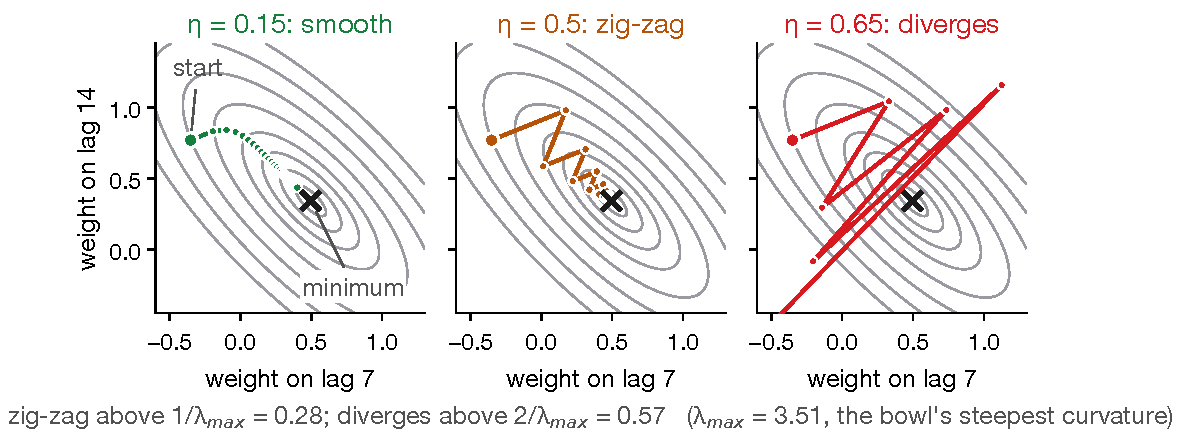
\includegraphics[height=4.6cm]{../Figures/Lecture07_NeuralNets/gd_bowl.pdf}
  \end{center}
  \vspace{-0.2cm}
  {\small The bowl is exact only because this model is linear: its curvature is the same
  everywhere, so $2/\lambda_{\max}$ is a hard limit. A network's loss surface curves differently
  in different places, one reason Adam adapts its step per parameter as it goes.}
\end{frame}

% --- Slide: Overfitting and regularization ------------------------------------
\begin{frame}{Preventing Overfitting --- Where Lecture 6 Returns}
  Twenty-two thousand parameters on five thousand rows will memorize the training set unless
  something stops it. Three things do, and \textbf{you have met two of them already}.

  \vspace{0.1cm}
  \begin{center}
    {\small
    \begin{tabular}{p{3.0cm}p{9.4cm}}
      \toprule
      \texttt{weight\_decay} & \textbf{This is Ridge.} An $\ell_2$ penalty on the weights, under
      a different name. \texttt{Adam(..., weight\_decay=1e-4)} \\[3pt]
      \texttt{nn.Dropout(p)} & Randomly zero a fraction $p$ of neuron outputs on each forward
      pass, so no neuron can depend on a specific other one being present. All neurons are
      active at test time. \\[3pt]
      Early stopping & Watch validation loss each epoch; stop when it has not improved for
      $k$ epochs, and keep the weights from the \emph{best} epoch, not the last. \\
      \bottomrule
    \end{tabular}
    }
  \end{center}

  \vspace{0.1cm}
  \textbf{That is the fifth appearance of one idea.} The GAM smoothing penalty in Lecture 3,
  cost-complexity pruning in Lecture 4, \texttt{reg\_lambda} on leaf weights in Lecture 5,
  Ridge and LASSO in Lecture 6 --- and now weight decay. Fit against complexity, one parameter
  setting the exchange rate, chosen by validation.
\end{frame}

% --- Slide: early stopping, measured ---------------------------------------------
\begin{frame}{Early Stopping, on Lab 7's Network}
  Lab 7's network, trained for 200 epochs instead of 60, three seeds:
  \begin{center}
    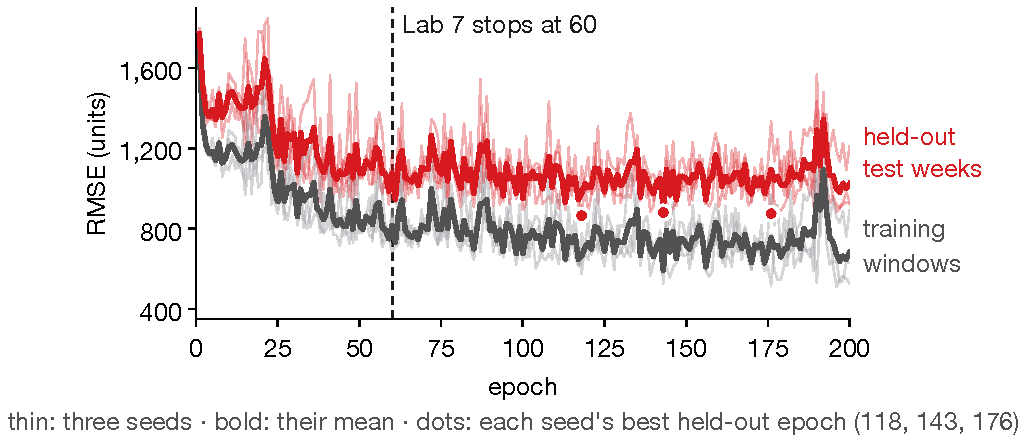
\includegraphics[height=4.7cm]{../Figures/Lecture07_NeuralNets/overfit_epochs.pdf}
  \end{center}
  \vspace{-0.3cm}
  {\small Training error keeps falling. Held-out error improves little after epoch 60 and jumps
  by about 100 from one epoch to the next, so \textbf{keep the best epoch, not the last}. Choose
  it on a validation slice cut from the training period, never on the test weeks drawn here.}
\end{frame}

% =============================================================================
\section{PyTorch Implementation}
% =============================================================================

\sectionslide{PyTorch Implementation}{%
  Four pieces: a Dataset, a DataLoader, a model, and a training loop.}

% --- Slide: PyTorch Dataset and DataLoader -----------------------------------
\begin{frame}{PyTorch: Dataset and DataLoader}
  \begin{examplebox}{Wrapping your arrays}
    {\tiny\linespread{1.2}\selectfont
    \texttt{from torch.utils.data import Dataset, DataLoader}\\[2pt]
    \texttt{class ForecastDataset(Dataset):}\\
    \texttt{\ \ def \_\_init\_\_(self, X, y):}\\
    \texttt{\ \ \ \ self.X = torch.tensor(X, dtype=torch.float32)}\\
    \texttt{\ \ \ \ self.y = torch.tensor(y, dtype=torch.float32)}\\
    \texttt{\ \ def \_\_len\_\_(self): return len(self.X)}\\
    \texttt{\ \ def \_\_getitem\_\_(self, i): return self.X[i], self.y[i]}\\[3pt]
    \texttt{loader = DataLoader(ForecastDataset(X\_tr, y\_tr),}\\
    \texttt{\ \ \ \ \ \ \ \ \ \ \ \ \ \ \ \ \ \ \ batch\_size=64, shuffle=False)}
    }
  \end{examplebox}
  \texttt{Dataset} fetches \emph{one} example; \texttt{DataLoader} batches.
  \textbf{\texttt{shuffle=False}} keeps runs identical. Shuffling these training windows would not
  leak the future --- each carries its own past; shuffling \emph{before} the time split would.
\end{frame}

% --- Slide: model definition -------------------------------------------------
\begin{frame}{PyTorch: Defining the Model}
  \begin{examplebox}{A two-layer network with dropout}
    {\scriptsize\linespread{1.15}\selectfont
    \texttt{import torch.nn as nn}\\[2pt]
    \texttt{model = nn.Sequential(}\\
    \texttt{\ \ \ \ nn.Linear(n\_features, 128), nn.ReLU(), nn.Dropout(0.3),}\\
    \texttt{\ \ \ \ nn.Linear(128, 128),\ \ \ \ \ \ nn.ReLU(), nn.Dropout(0.3),}\\
    \texttt{\ \ \ \ nn.Linear(128, 1))}
    }
  \end{examplebox}
  Read it top to bottom and it is the block diagram from \emph{How Big Is This Model?}: a linear
  map, a nonlinearity, some dropout, again, then a linear output with no activation.

  \vspace{0.15cm}
  \texttt{nn.Sequential} chains layers in order and is enough for anything in this lecture. When
  an architecture needs branching or a skip connection --- Lecture 8 --- you subclass
  \texttt{nn.Module} and write \texttt{forward()} yourself.

  \vspace{0.15cm}
  \muted{\footnotesize\itshape \texttt{nn.Linear(in, out)} holds the weight matrix and bias for
  one layer. That is where the 22{,}657 parameters live.}
\end{frame}

% --- Slide: training loop ----------------------------------------------------
\begin{frame}{PyTorch: The Training Loop}
  \begin{examplebox}{The four steps, per mini-batch}
    {\tiny\linespread{1.2}\selectfont
    \texttt{opt = torch.optim.Adam(model.parameters(), lr=1e-3, weight\_decay=1e-4)}\\
    \texttt{lossfn = nn.MSELoss()}\\[3pt]
    \texttt{for epoch in range(n\_epochs):}\\
    \texttt{\ \ model.train()}\\
    \texttt{\ \ for xb, yb in loader:}\\
    \texttt{\ \ \ \ opt.zero\_grad()\ \ \ \ \ \ \ \ \ \ \ \ \ \ \# 1 clear old gradients}\\
    \texttt{\ \ \ \ loss = lossfn(model(xb).squeeze(), yb)\ \# 2 forward}\\
    \texttt{\ \ \ \ loss.backward()\ \ \ \ \ \ \ \ \ \ \ \ \ \ \# 3 backward}\\
    \texttt{\ \ \ \ opt.step()\ \ \ \ \ \ \ \ \ \ \ \ \ \ \ \ \ \# 4 update weights}
    }
  \end{examplebox}
  Every PyTorch training loop is those four lines with more around them.

  \vspace{0.1cm}
  \textbf{The one that bites:} forget \texttt{zero\_grad()} and PyTorch \emph{accumulates} gradients
  rather than replacing them. No error, no warning --- just a model that trains badly.
\end{frame}

% =============================================================================
\section{Key Takeaways}
% =============================================================================

\sectionslide{Key Takeaways}{%
  Where a network belongs in the toolkit you now have.}

% --- Slide: comparison -------------------------------------------------------
\begin{frame}{Neural Networks vs.\ Tree Methods \parencite{James2021}}
  \begin{center}
    {\small
    \begin{tabular}{lllll}
      \toprule
      \textbf{Method} & \textbf{Sequences} & \textbf{Extrapolates} & \textbf{Tuning} & \textbf{Best for} \\
      \midrule
      LASSO / Ridge & no & yes & light & Many correlated predictors \\
      Random forest & no & no & light & Tabular, robust default \\
      XGBoost & no & no & moderate & Tabular, best-in-class \\
      FFN & no & yes & heavy & Smooth functions, large $n$ \\
      RNN / LSTM & \textbf{yes} & yes & heavy & Sequences (Lecture 9) \\
      \bottomrule
    \end{tabular}
    }
  \end{center}

  \vspace{0.15cm}
  \textbf{An FFN on lag features is doing the same job as XGBoost on lag features} --- same
  inputs, same flat table, no notion of order. It is not obviously the better tool, and on the
  evidence of Homework 4 it usually is not.

  \vspace{0.15cm}
  What changes in the next two lectures is the \emph{architecture}: convolutions that see local
  structure, and recurrence that carries state through time. That is when the sequence column
  above starts saying yes, and it is the reason to learn this machinery now.
\end{frame}

% --- Slide: Key takeaways ---------------------------------------------------
\begin{frame}{Lecture 7: Key Takeaways}
  \begin{keybox}
    {\footnotesize
    \begin{enumerate}\itemsep2pt
      \item A \textbf{neuron} is regression inside a nonlinearity; with ReLU, each unit adds a
            kink.

      \item Width and depth set an \textbf{FFN}'s capacity: 22{,}657 parameters on 5{,}000
            rows.

      \item \textbf{Training}: loss $\to$ \texttt{backward()} $\to$ \texttt{step()}, per
            mini-batch; keep the best epoch.

      \item \textbf{Regularization is not new}: weight decay is Ridge.

      \item For time series: split by time, \textbf{never shuffle before the split}, call
            \texttt{zero\_grad()} every batch.

      \item An FFN on engineered features competes with XGBoost; it is \textbf{not an upgrade}.
    \end{enumerate}
    }
  \end{keybox}
  \muted{\itshape Next: convolutions, including 1D ones for time series.}
\end{frame}

% --- References ---------------------------------------------------------------
\begin{frame}[allowframebreaks]{References}
  \printbibliography[heading=none]
\end{frame}

% =============================================================================
\end{document}
% =============================================================================
